\documentclass[preview]{standalone}

% tikz
\usepackage{tikz}
\usetikzlibrary{intersections, angles, quotes, positioning}
\usetikzlibrary{arrows.meta}
\usepackage{pgfplots}
\pgfplotsset{compat=1.13}
\tikzset{
	force/.style={thick, {Circle[length=2pt]}-stealth, shorten <=-1pt}
}

\begin{document}
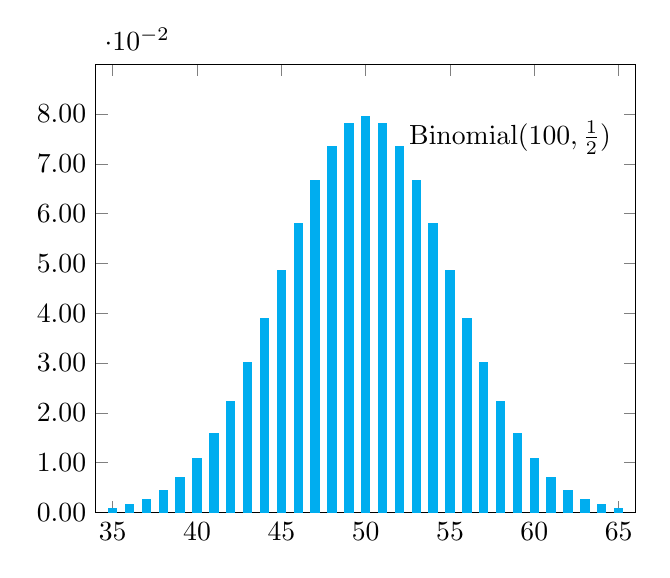
\begin{tikzpicture}
    \begin{axis}
    [
        % Define probability distribution functions
        declare function={
            binom(\n,\p) = \n!/(x!*(\n-x)!)*\p^x*(1-\p)^(\n-x);
            normal(\m,\s) = 1/(\s*sqrt(2*pi))*exp(-((x-\m)^2)/(2*\s^2));
        },
        % Plotting options
        xmin=34, xmax=66,
        ymin=0.0, ymax=0.09,
        samples at={35,...,65},
        xtick={35,40,...,65},
        ytick={0,0.01,...,0.08},
        yticklabel style={
            /pgf/number format/fixed,
            /pgf/number format/fixed zerofill,
            /pgf/number format/precision=2,
        },   
    ]
    
    % Plot Binomial Distribution
    \addplot [draw=cyan,ybar=0pt,bar width=3pt,fill=cyan] {binom(100,0.5)};
    % Add "discrete CDF" label
    \node[anchor=south west] at (axis cs:52,0.07) {Binomial(\(100, \frac{1}{2}\))};
    \end{axis}
    \end{tikzpicture}
\end{document}